\documentclass[runningheads]{llncs}

\usepackage[margin=1.5in]{geometry}
\usepackage{amsmath}
\usepackage{amssymb}
\usepackage{mathrsfs}  
\usepackage{lipsum}
\usepackage{comment}
\usepackage{graphicx}
\usepackage{framed}
\usepackage{setspace}
\setlength\FrameSep{1em}
\setlength\OuterFrameSep{\partopsep}
% \usepackage{authblk}
\usepackage[modulo]{lineno}
\linenumbers
\usepackage{xargs}                      % Use more than one optional parameter in a new commands
\usepackage[pdftex,dvipsnames]{xcolor}  % Coloured text etc.
\usepackage[colorinlistoftodos,prependcaption,textsize=tiny]{todonotes}
\newcommandx{\XXXunsure}[2][1=]{\todo[linecolor=red,backgroundcolor=red!25,bordercolor=red,#1]{#2}}
\newcommandx{\XXXchange}[2][1=]{\todo[linecolor=blue,backgroundcolor=blue!25,bordercolor=blue,#1]{#2}}
\newcommandx{\XXXinfo}[2][1=]{\todo[linecolor=OliveGreen,backgroundcolor=OliveGreen!25,bordercolor=OliveGreen,#1]{#2}}
\newcommandx{\XXXimprovement}[2][1=]{\todo[linecolor=Plum,backgroundcolor=Plum!25,bordercolor=Plum,#1]{#2}}
\newcommandx{\XXX}[2][1=]{\todo[disable,#1]{#2}}
\usepackage{fancyhdr}
\newcommandx{\AVATokenName}{\texttt{\$AVAX}}
\newcommandx{\AVAPlatformName}{\texttt{Avalanche}}
\newcommandx{\AVAPlatformNameFirstRelease}{\texttt{Avalanche BOREALIS}}
\newcommandx{\genericAvalanche}{$\mathtt{A}^{*}$}
\usepackage[yyyymmdd,hhmmss]{datetime}
\newcommand\ddfrac[2]{\frac{\displaystyle #1}{\displaystyle #2}}

\setlength{\parindent}{2.0em}
\setlength{\parskip}{1.0em}
\renewcommand{\baselinestretch}{1.25}

\fboxsep=1pt%padding thickness
\fboxrule=0.2pt%border thickness

\begin{document}

\immediate\write18{git rev-parse HEAD > /tmp/temp.dat}

\title{\AVAPlatformName{} Native Token (\AVATokenName{}) Dynamics \\\today}
\author{Stephen Buttolph, Amani Moin, Kevin Sekniqi, and Emin G{\"u}n Sirer}
\institute{}

\maketitle

\begin{abstract}
% The Avalanche paper~\cite{avalanche} introduced a novel family of consensus protocols based repeated subsampled voting. 
% While Avalanche achieves high scalability, high throughput, and low latency with a green, sustainable footprint, the original paper does not by itself define a specific currency implementation. 

This paper discusses the key implementation details, in particular the token economics (tokenomics), of the native token of the \AVAPlatformName{} platform, called \AVATokenName{}. The native token secures the network, pays for fees, and provides the basic unit of account between the multiple blockchains deployed on the larger \AVAPlatformName{} network. 
% XXX MOVE In aggregate, these features make \AVAPlatformName{} the most robust, performant, and feature-packed platform for reaching a broad base of users and for serving as a foundation for internet-scale public blockchain platform.
For additional details on \AVAPlatformName{}, which serves as a versatile and universal platform, allowing anyone to launch new blockchains with their own rules, virtual machines, and validator sets, we guide the reader to either the accompanying architectural paper~\cite{avaplatformpaper} or the \AVAPlatformName{} docs~\cite{avadocs}.

\end{abstract}
\begin{center} 
   \scriptsize Git Commit: \input{/tmp/temp.dat}
\end{center}

\noindent{\setstretch{0.5}\scriptsize\underline{Disclosure:} The information described in this paper is preliminary and subject to change at any time. Furthermore, this paper may contain “forward-looking statements”. Forward-looking statements generally relate to future events or our future performance. This includes, but is not limited to, \AVAPlatformName{}'s projected performance; the expected development of its business and projects; execution of its vision and growth strategy; and completion of projects that are currently underway, in development or otherwise under consideration. Forward-looking statements represent our management’s beliefs and assumptions only as of the date of this presentation. These statements are not guarantees of future performance and undue reliance should not be placed on them. Such forward-looking statements necessarily involve known and unknown risks, which may cause actual performance and results in future periods to differ materially from any projections expressed or implied herein. \AVAPlatformName{} undertakes no obligation to update forward-looking statements. Although forward-looking statements are our best prediction at the time they are made, there can be no assurance that they will prove to be accurate, as actual results and future events could differ materially. The reader is cautioned not to place undue reliance on forward-looking statements.}
    

\section{Introduction}
The economic model of any new digital currency/asset is one of the most critical components of the platform that the asset resides on. This is especially true for the native token of a self-sovereign, permission-less platform, like \AVAPlatformName{}. In this paper, we discuss the economic design of the native token, called \AVATokenName{}. The discussion is broken down into the governance properties of the token, its supply, minting (rewards) function of stakers, and other pertinent economics details, such as the transactional economy. 
% {\color{red} We also include a discussion of the economic pros and cons of proof-of-stake and proof-of-work.\XXXunsure{Should we really talk about this? We will *not* win people over by going against PoW. It doesn't even seem like our fight to win. What does it buy us?}}

\subsection{Key \AVATokenName{} Properties}
These are the key takeaway properties of the design of the \AVATokenName{} economics model:

\begin{itemize}
    \item The resources spent by a validator for staking are proportional to that validator's total stake. 
    \item The rewards accumulated by a validator for validating are proportional to that validator's total stake. 
    \item Since \AVAPlatformName{} is leaderless, there is no ``rich-get-richer'' compounding effects.
    \item Validators that lock their stake for longer are rewarded more.
    \item Validators are incentivized to stay online and operate correctly as their rewards are based on proof-of-uptime and proof-of-correctness.
    \item \AVATokenName{} is a capped-supply token, with a maximum cap of $720$ million tokens.
    \item While capped, \AVATokenName{} is still governable. The rate at which the maximum cap is reached is subject to governance. 
    \item Fees are not paid to any specific validator. Instead, they are burned, thus increasing scarcity of the \AVATokenName{}. 
\end{itemize}

\section{Governance}
We initiate our survey of the \AVAPlatformName{} economic design by first discussing governance, as it plays a critical role within future components. To enable the system to adapt to changing economic conditions, the \AVAPlatformName{} platform enables key system parameters to be modified dynamically based on user input. 
A workable process for finding globally acceptable values for system parameters is critical for decentralized systems without custodians. 
\AVAPlatformName{} can use its consensus mechanism to build a system that allows anyone to propose special transactions that are, in essence, system-wide polls. 
Any participating node may issue such proposals. 

Reward rate is an important parameter that affects any currency, whether digital or fiat. 
Unfortunately, cryptocurrencies that fix this parameter might face various issues, including deflation or hyper-inflation.
To that end, the reward rate will be subject to governance, within pre-established boundaries. This will allow token holders to choose the rate at which \AVATokenName{} reaches its capped supply. 

Transaction fees, denoted by the set $\mathcal{F}$, will also be eventually be governed. 
$\mathcal{F}$ is effectively a tuple which describes the fees associated with the various instructions and transactions supported in future releases. 
Finally, staking times and amounts will also be governable. 
The list of these parameters is defined in Figure~\ref{fig:notation}.

\begin{figure}[hbtp]
\begin{framed}
\begin{itemize}
\item{$\Delta$} : Staking amount, denominated in \AVATokenName{}. This value defines the minimal stake required to be placed as bond before participating in the system. The default value on genesis will be 2,000 \AVATokenName{}.
% \item{$\bar{f}$} : The minimal time before a node can request to mint new coins, calculated as elapsed time since last minting event. 
\item{$\delta_{min}$} : The minimal amount of time required for a node to stake into the system. The default value on genesis will be 2 weeks.
\item{$\delta_{max}$} : The maximal amount of time a node can stake. The default value on genesis will be 52 weeks.
% \item{$\rho: (\pi\Delta,\tau\delta_{min}) \rightarrow \mathbb{R}$} : Interest rate function, also referred to as minting rate, determines the reward a participant can claim as a function of their staking amount given some number of $\pi$ publicly disclosed nodes under its ownership, over a period of $\tau$ consecutive $\delta_{min}$ timeframes, such that $\tau\delta_{min} \leq \delta_{max}$. 
\item{$\gamma, \lambda$} : The two key parameters in governing the minting rate function. 
\item{$\mathcal{F}$} : the fee structure, which is a set of governable fees parameters that specify costs to various transactions.
\end{itemize}
\end{framed}
\caption{Key governable parameters used in \AVAPlatformName{}.}
\label{fig:notation}
\end{figure}

Ultimately, we note that governance in \AVATokenName{} has hysteresis, meaning that changes to parameters are highly dependent on their recent changes. There are two limits associated with each governable parameter: time and range. Once a parameter is changed using a governance transaction, it becomes very difficult to change it again immediately and by a large amount.  These difficulty and value constraints relax as more time passes since the last change. These restrictions are in keeping with the design philosophy of predictability: the system must never change drastically over a short period of time, allowing users to safely predict system parameters in the short term, while having strong control and flexibility for the long term.

\section{Token Economics}

\AVATokenName{} has a capped-supply of 720,000,000 (720M) tokens. The genesis block will have 360M \AVATokenName{} tokens. The rest of the  360M tokens will be minted according to Equation~\ref{eq:minting-function}. For a graphical representation, Figure~\ref{fig:mintingfunction-graph} shows the token emissions curve between \AVATokenName{} and BTC. The principle of the emissions function chosen for \AVAPlatformName{} is simple: reach a capped supply, in a fashion similar to Bitcoin's emissions curve, and yet maintain the ability to govern the rate at which the system reaches this limit.

\subsection{Minting Function}

$R_j$ is total number of tokens at year $j$, with $R_1 = 360M$, and $R_l$ representing the last year that the values of $\gamma, \lambda \in \mathbb{R}$ were changed; $c_j$ is the yet un-minted supply of coins to reach $720M$ at year $j$ such that $c_j \leq 360M$; $u$ represents a staker, with $u.s_{amount}$ representing the total amount of stake that $u$ possesses, and $u.s_{time}$ the length of staking for $u$.

\begin{equation}
R_j = R_{l} + \sum_{\forall u} \rho(u.s_{amount}, u.s_{time}) \times (c_j/L) \times \left(\sum\limits_{i=0}^{j}\ \ddfrac{1}{\left(\gamma + \ddfrac{1}{1 + i^{\lambda}}\right)^i} \right)
\label{eq:minting-function}
\end{equation}
where, 
\begin{equation}
L = \left(\sum\limits_{i=0}^{\infty}\ \ddfrac{1}{\left(\gamma + \ddfrac{1}{1 + i^{\lambda}}\right)^i}\right)
\end{equation}
At genesis, $c_1 = 360M$. The values of $\gamma$ and $\lambda$ are governable, and if changed, the function is recomputed with the new value of $c_{*}$. We have that $\sum_{*} \rho(*) \leq 1$. $\rho(*)$ is a linear function that can be computed as follows ($u.s_{time}$ is measured in weeks, and $u.s_{amount}$ is measured in \AVATokenName{} tokens): 
\begin{equation}
\rho(u.s_{amount}, u.s_{time}) = (0.002\times u.s_{time} + 0.896) \times \frac{u.s_{amount}}{R_j}
\end{equation}
If the entire supply of tokens at year $j$ is staked for the maximum amount of staking time (one year, or 52 weeks), then $\sum_{\forall u} \rho(u.s_{amount}, u.s_{time}) = 1$. If, instead, every token is staked continously for the minimal stake duration of two weeks, then $\sum_{\forall u} \rho(u.s_{amount}, u.s_{time}) = 0.9$. Therefore, staking for the maximum amount of time incurs an additional 11.11\% of tokens minted, incentivizing stakers to stake for longer periods. Due to the capped-supply, the function above guarantees that regardless of the number of governance changes, we will never exceed a total of $720M$ tokens. Therefore, 
\begin{equation}
    \lim_{j = \infty} R_j = \text{720M}
\end{equation}

\begin{figure}[h!]
\centering
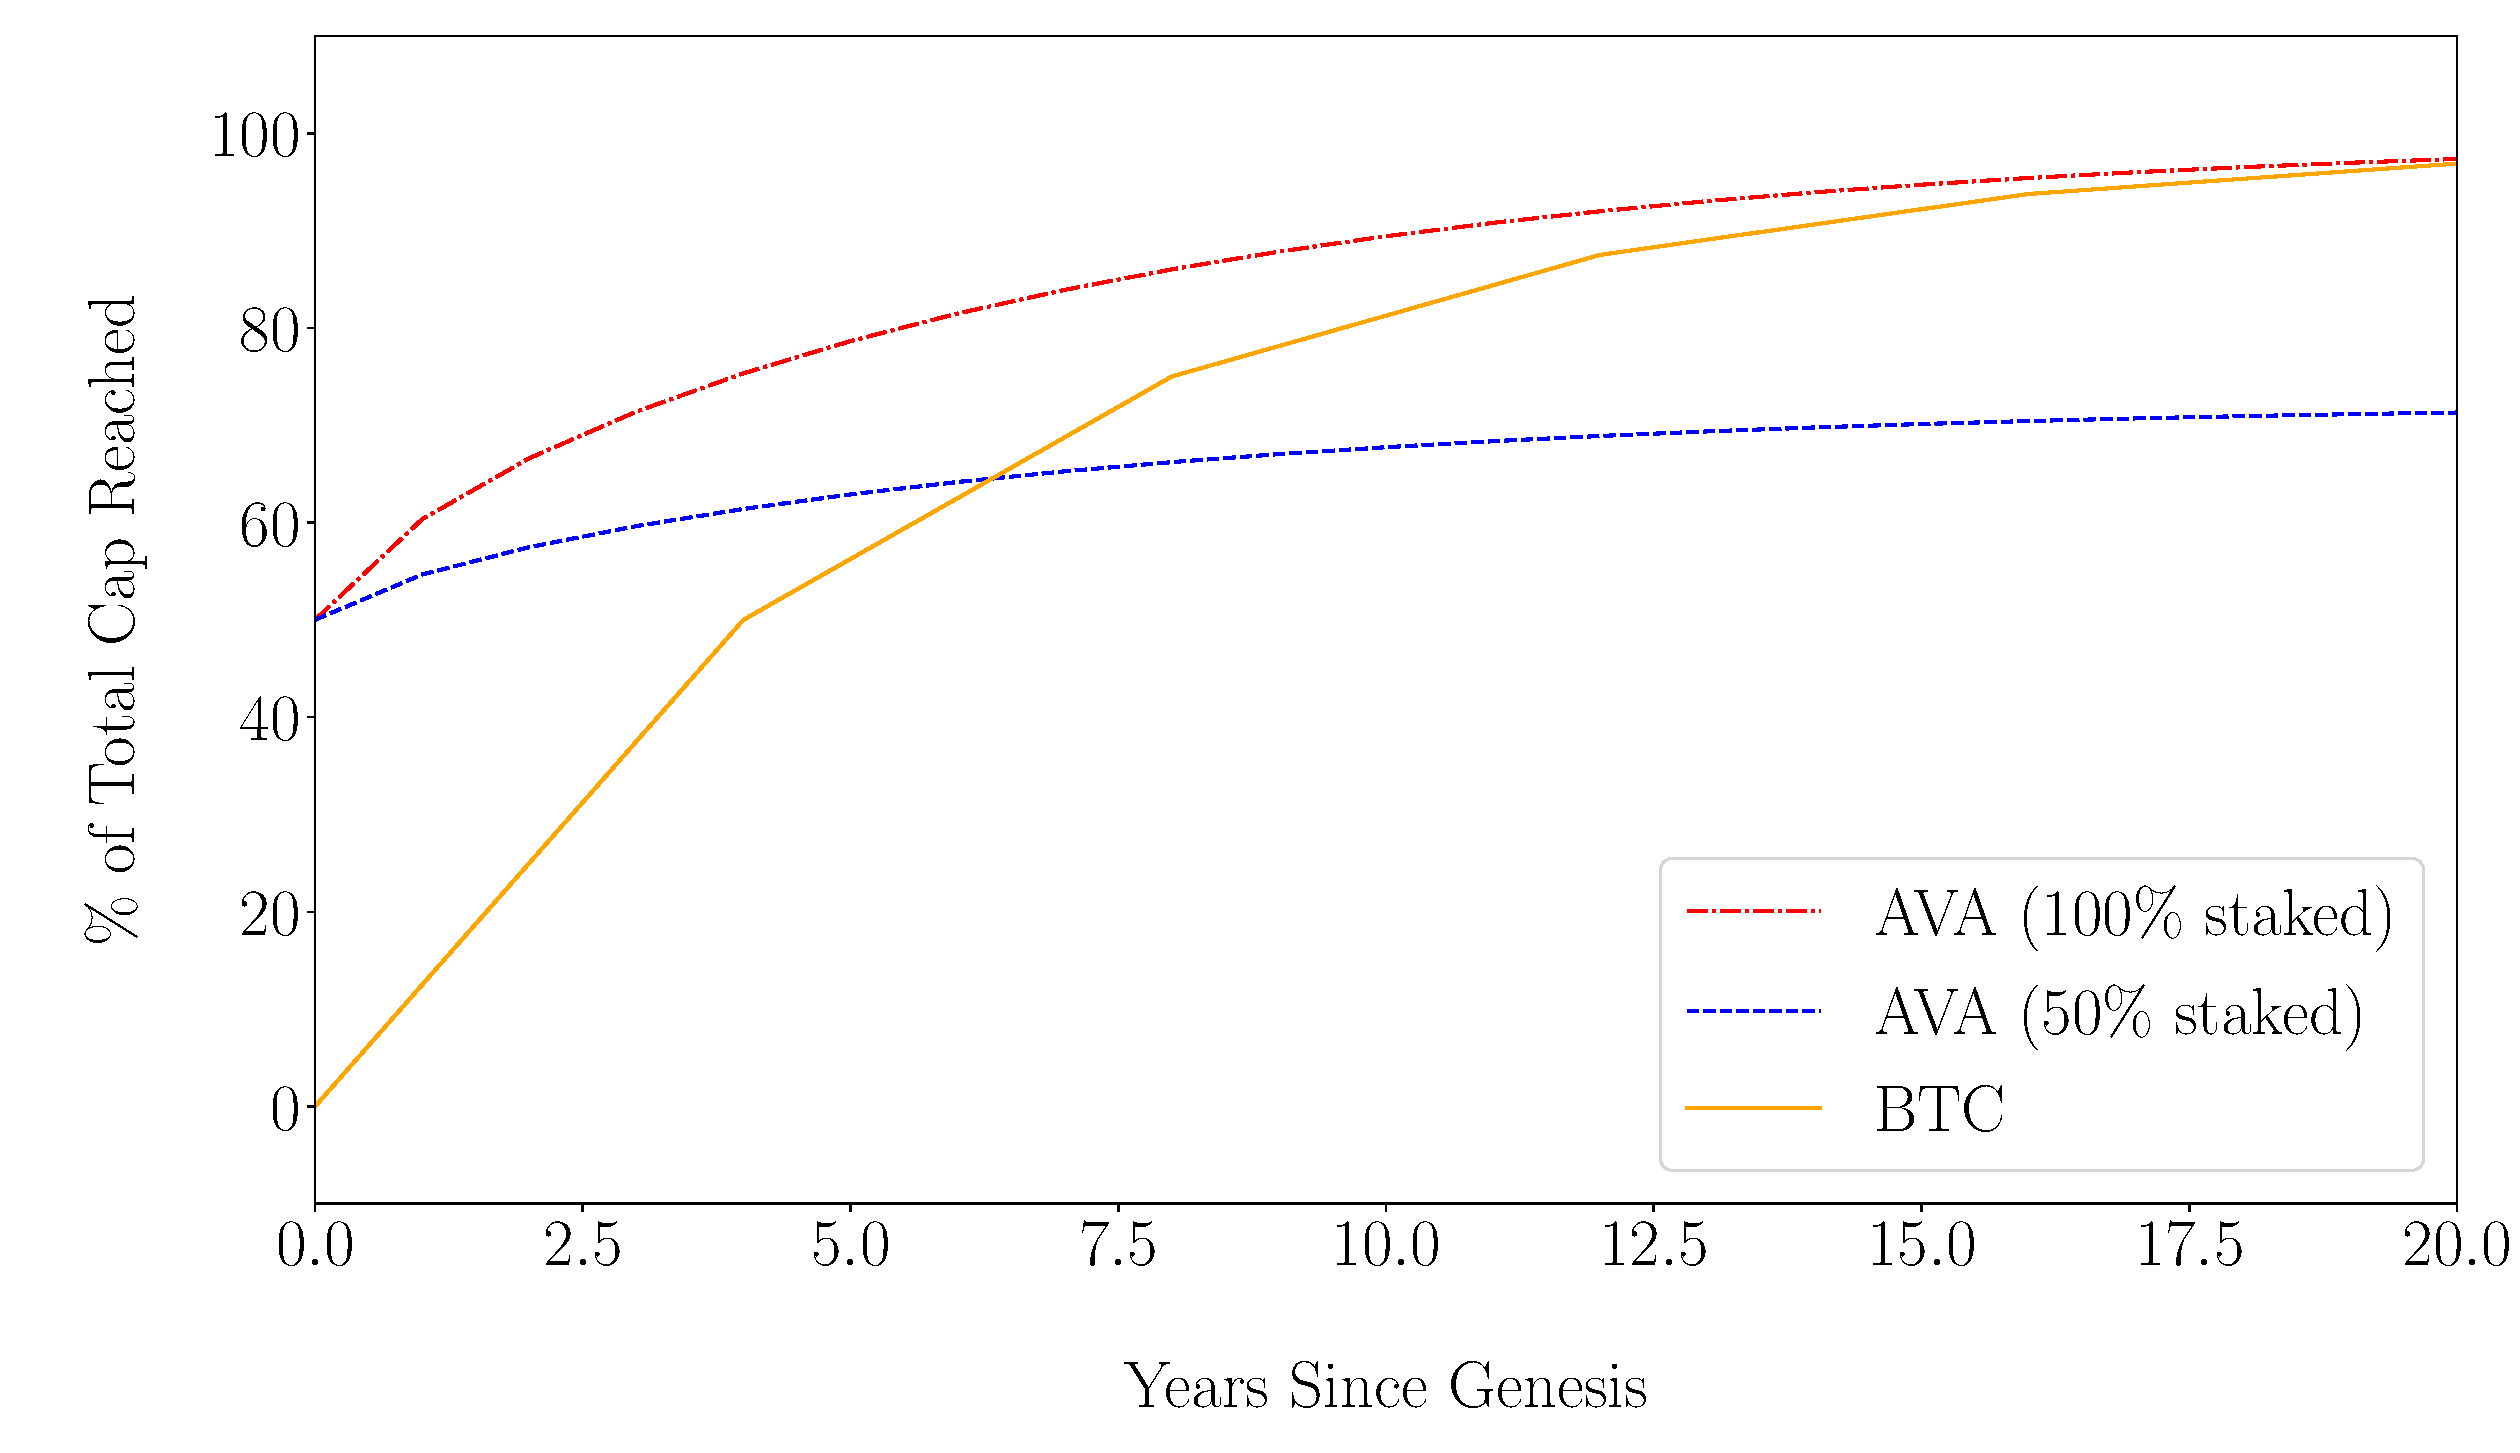
\includegraphics[width=\linewidth]{./mintingfunction_20years.pdf}
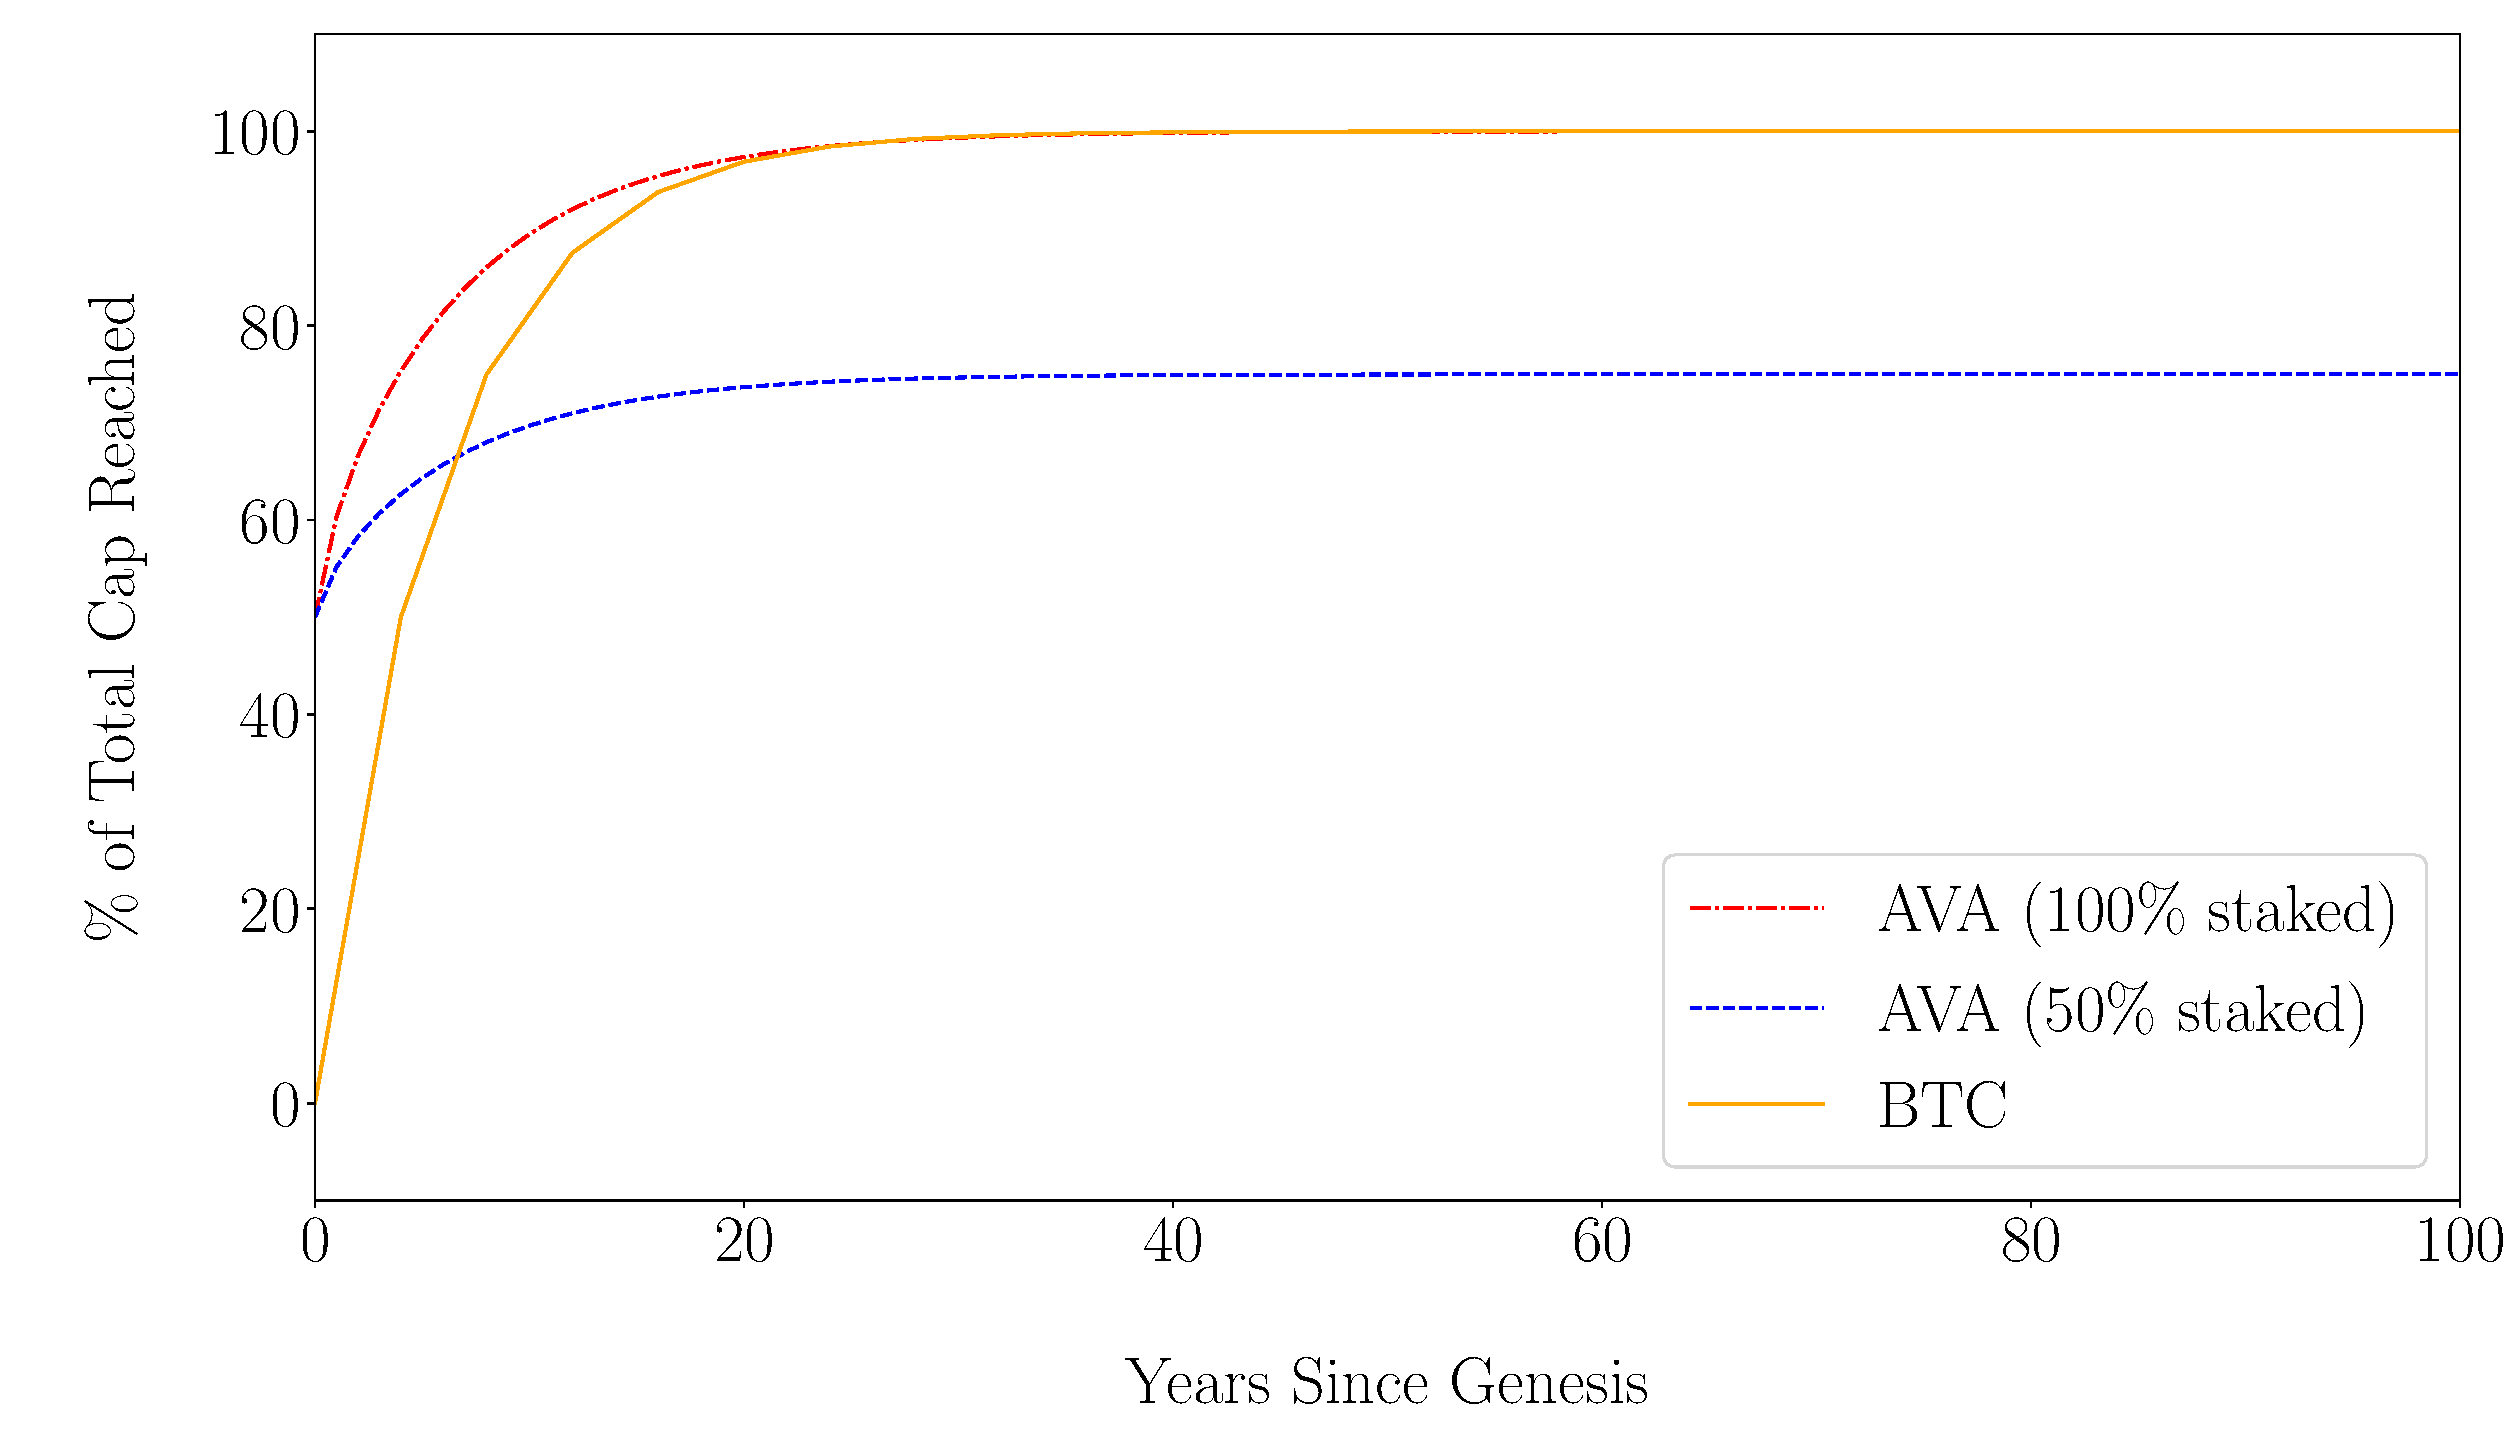
\includegraphics[width=\linewidth]{./mintingfunction_100years.pdf}
\caption{Token emissions between \AVATokenName{} and BTC, calculated over a 20 year and 100 year horizon, with $\gamma = 1.15$ and $\lambda=1.1$. The curve for ``\AVATokenName{} (100\% staked)'' represents the case where every token is being staked repeatedly for the maximum staking duration of one year, i.e. $\sum_{\forall u} \rho(u.s_{amount}, u.s_{time}) = 1$. On the other hand, the curve of ``\AVATokenName{} (lower)'' represents the case where only 50\% of the tokens are being staked repeatedly over the minimal staking duration of two weeks, i.e. $\sum_{\forall u} \rho(u.s_{amount}, u.s_{time}) = 0.45$. We note that, for simplicity, these graphs represent the case where $\gamma$ and $\lambda$ are fixed at genesis and never governed afterwards. The goal of changing $\gamma$ and $\lambda$ is to increase total supply of tokens in case the empirically observed total staked supply is too low.}
\label{fig:mintingfunction-graph}
\end{figure}
\clearpage
\section{Minting Mechanism}
Minting in \AVATokenName{} is designed to incentivize nodes to behave in a way that positively helps global outcomes. This is accomplished by special \emph{minting transactions}. A node earns the right to mint by first putting up a stake and then participating actively in the consensus process. 
Specifically, node rewards are directly linked to their uptime and response latency. Every node maintains local information about the liveness and behavior of each other node with which it interacted. Whenever a node $v$ is sampled by $u$, the latter maintains a local tuple of (response bit, timestamp). 
The first entry is a single bit representing whether $v$ responded within the timeout, and the second represents the timestamp of the response. 
In other words, minting in \AVAPlatformName{} is done via proof-of-uptime and proof-of-responsiveness. 
This mechanism has important consequences. In particular, since there is no ``leader'' accumulating rewards, there is no ``rich-get-richer'' compounding effects. 

% This minting/reward function, unique to \AVATokenName, is defined next.
% \subsubsection{Reward Function}
% \begin{figure}[h!]
%     \centering
%     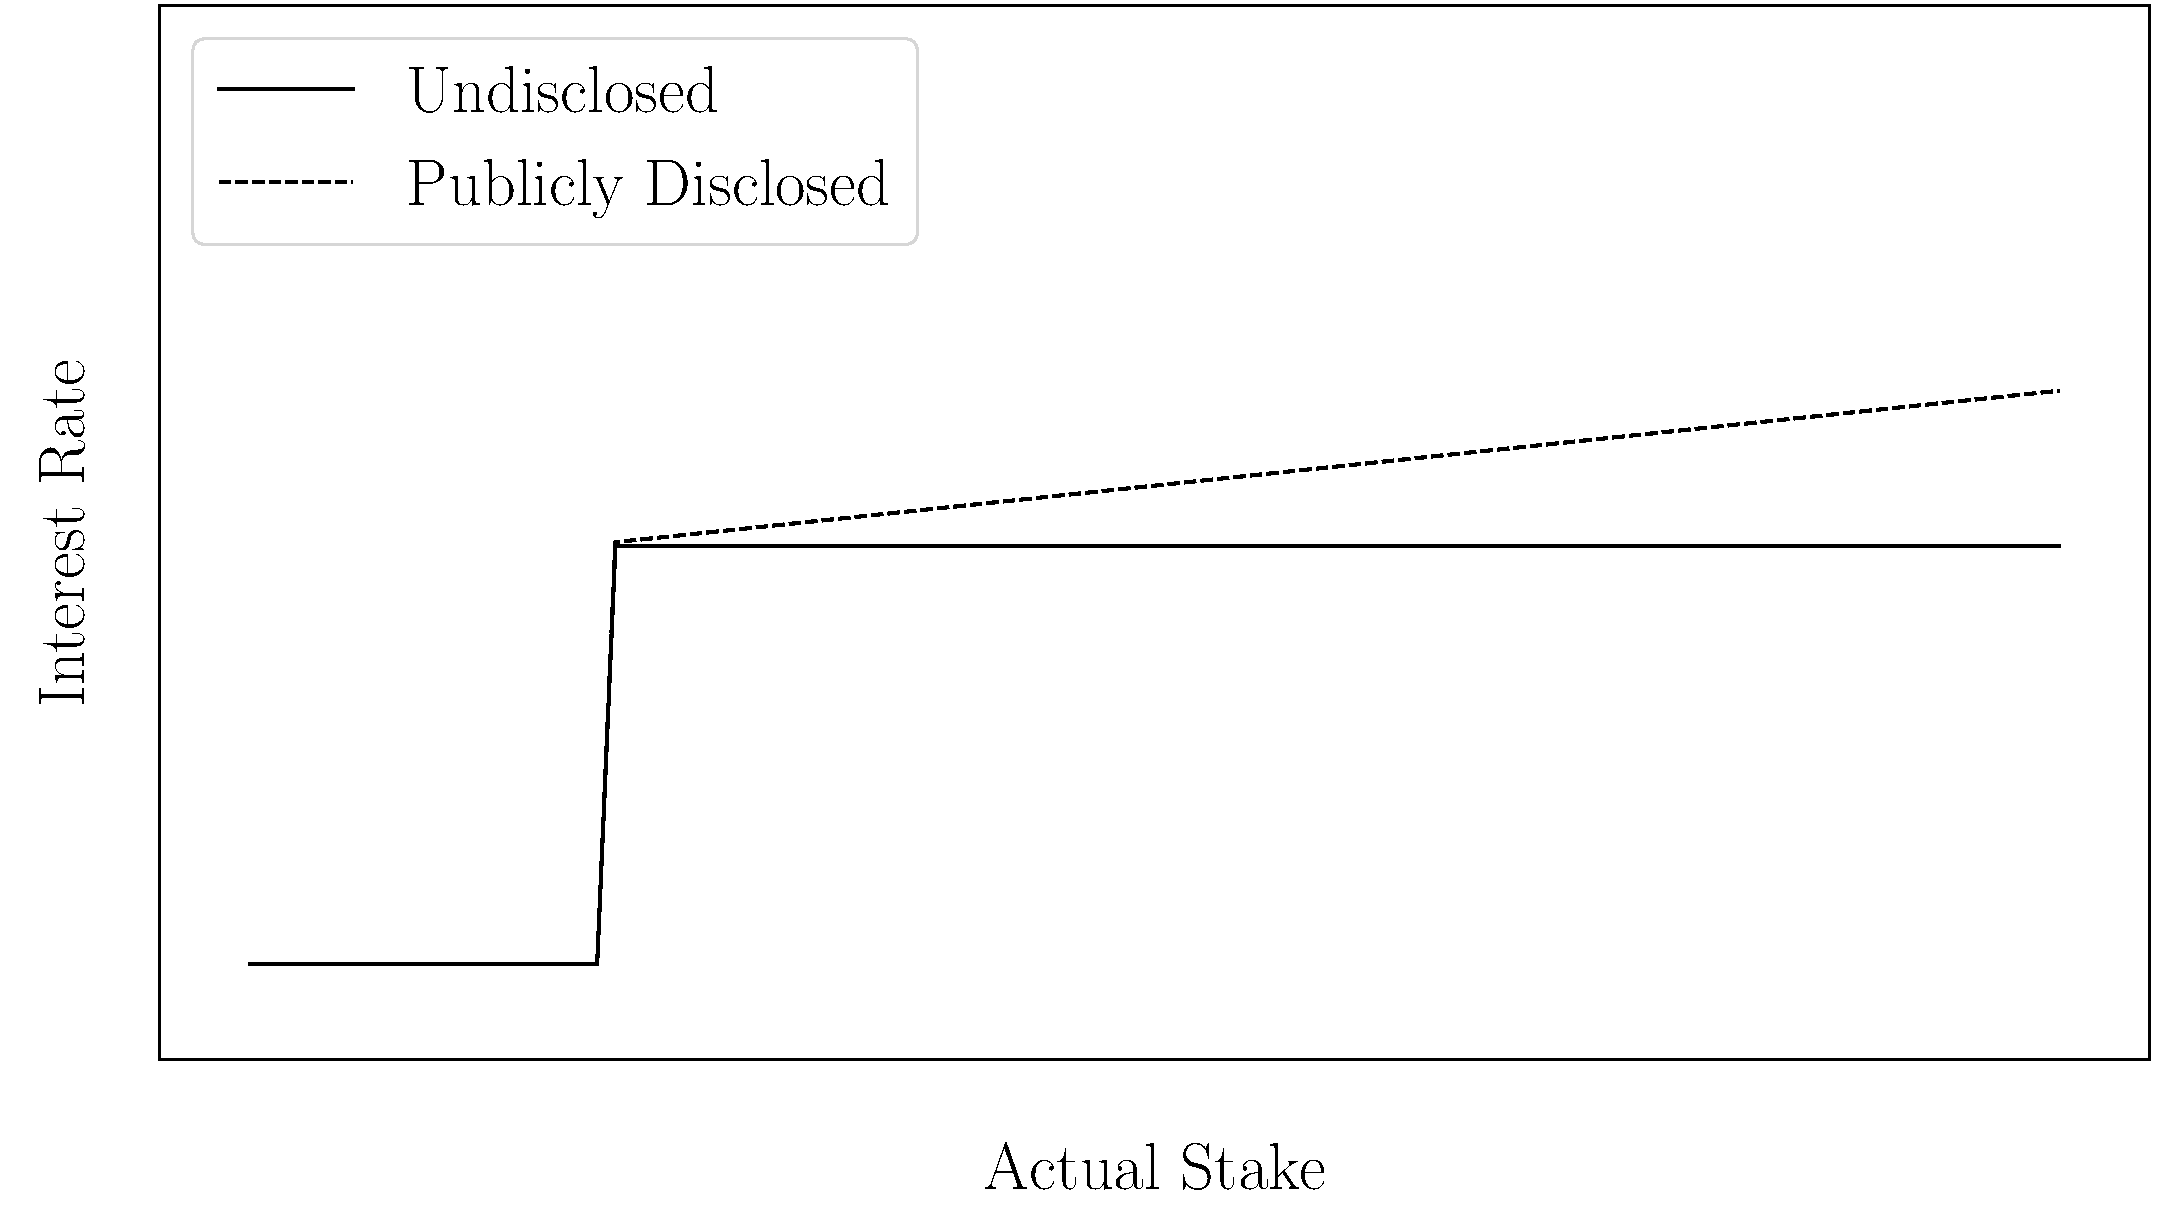
\includegraphics[width=0.6\linewidth]{./reward_function.pdf}
%     \caption{Interest rate as a function of actual stake in the system. The steep step point is $\Delta$. In \AVATokenName, nodes that disclose all nodes under ownership receive a slightly higher reward than nodes which may keep such information private.}
%     \label{fig:rewardfunction}
%     \end{figure}
% The minting (interest) rate is set up as function $\rho$.
% The reward is exactly zero if a node stakes less than the minimal required threshold, and scales as a multiple of the minimum stake. 

% The reward also scales monotonically with the length of time that coins are staked.  

% In addition to minting as a reward for participation in the consensus protocol, we can also reward users for other types of engagement, such as contributing positively to the \AVAPlatformName{} ecosystem.  We anticipate implementing these rewards as use it or lose it coins, wherein we would airdrop coins to particular keys; these coins would vanish or revert back to another address if not claimed or used before a set amount of time.  This ensures the coins are being distributed to active users and avoids tying up more coins in inactive accounts. Destroying coins not used before a particular time can also be used to stimulate economic activity, as people will be disinclined to let the coins go to waste.    

\section{Transaction Economy}
\subsection{Fees Structure}
The fee structure in the \AVAPlatformName{} platform carries several differentiating features that distinguish it from other existing and upcoming platforms. 

\paragraph{Staker Fees.} Unlike other protocols that pay all fees to the elected leader, such as in Bitcoin, in \AVAPlatformName{} fees are simply burned. 
Therefore, payment is global and for the good of the entire ecosystem. Fee burning increases scarcity of tokens in the system. The minting process offsets the transaction fee burning, therefore there is no danger of the system grinding to a long term halt due to gradual destruction of coins. 
\paragraph{Transaction Costs.} In \AVAPlatformName{}, transaction fees differ depending on the type of transaction. 
Instantiations of new subnetworks carry the heaviest fees. 
In contrast, other types of transactions, such as simple payments of \AVATokenName{}, carry little cost. 
For other subnets, transactions pay fees in that subnet's native token, as well as some amount in the \AVATokenName{} token. 
A transaction native to a subnetwork may specify its own transaction fee structure, and it is up to the creator of the subnet to choose a fee structure that incentivizes validation for open, permissionless subnetworks.
\paragraph{Sliding Cost Function.} Transaction fees carry a sliding-cost function. 
The fee is not set by the issuer of the transaction, but rather by a globally verifiable fee-function. 
As the congestion in the network increases, fees increase. 
At the end of some specific period of time, the function is recalculated to accommodate natural increases in transaction volume in the network.
% Figure \ref{fig:transactionfees} shows this trend.
\paragraph{Transaction Tiers.} Unlike in a model such as Ethereum's, where every transaction invocation must pay some gas, \AVAPlatformName{} adopts a different model that incorporates two types of transaction processing mechanisms. 
All keys with positive account balances will be able to immediately interact with the platform, where the fees will be based on an allotment mechanism, functionally similar to a tiered payments model adopted in cloud computing platforms. 
Every transaction will name a sender address (i.e. the invoker), which will be checked for current invocation allotment. 
If the address still has free invocations left, the transaction does not have to carry any fees attached by the sender. 
Past a certain amount of calls, the sender will need to attach some fees based on the resources used to compute the transaction. 
Additionally, users may opt instead pay for their transactions using computation. 
To that end, future releases will support free frequency-limited transactions, which do not require fees in coins but require some pre-computation. 
Whenever a new transaction is generated, the user will compute and attach a valid PoW on the transaction, which can be checked by all other parties.

\subsection{Spam Management}
Although simple payments do carry fees, the value will be virtually zero. This, however, can lead to spam in the network. 
In future releases, to prevent congestion, each transaction carries with it a local PoW. 
The PoW is initially of low difficulty and therefore a transaction can be immediately issued with very little overhead. 
However, if a specific key generates a large amount of transactions in a short amount of time, each subsequent transaction will carry a larger amount of difficulty in its PoW puzzle. 
This mechanism works in conjunction with the fee burning. 

\bibliography{ava-token}
\bibliographystyle{splncs04}
\end{document}
